% 2013 年安徽卷理科第 15 题：正方体 ABCD-A1B1C1D1，P 为 BC 中点，Q 在 CC1 上。
% 来源 PDF：普通高考/2013/2013安徽理.pdf，第 1 页（印面 783）右栏上部。
% 斜二测投影：screen(x,y,z) = (2.2x + 1.0y, 0.62y + 2.2z)，棱长 1。
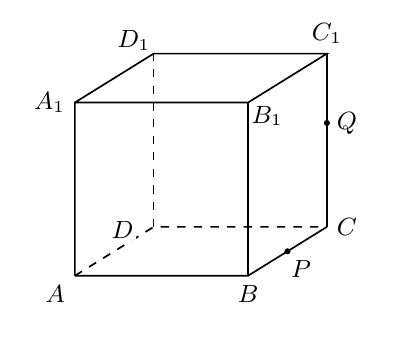
\begin{tikzpicture}[semithick, font=\small]
  \useasboundingbox (-0.6,-0.6) rectangle (3.8,3.15);
  \coordinate (A)  at (0,0);
  \coordinate (B)  at (2.2,0);
  \coordinate (C)  at (3.2,0.62);
  \coordinate (D)  at (1.0,0.62);
  \coordinate (A1) at (0,2.2);
  \coordinate (B1) at (2.2,2.2);
  \coordinate (C1) at (3.2,2.82);
  \coordinate (D1) at (1.0,2.82);
  \coordinate (P)  at (2.7,0.31);
  \coordinate (Q)  at (3.2,1.94);
  % 可见棱
  \draw (A) -- (B) -- (C);
  \draw (A) -- (A1) -- (B1) -- (C1) -- (D1) -- (A1);
  \draw (B) -- (B1);
  \draw (C) -- (C1);
  % 被遮挡的棱
  \draw[dashed] (A) -- (D) -- (C);
  \draw[dashed] (D) -- (D1);
  % 点 P、Q
  \fill (P) circle (1.1pt);
  \fill (Q) circle (1.1pt);
  % 标注
  \node[below left] at (A) {$A$};
  \node[below] at (B) {$B$};
  \node[right] at (C) {$C$};
  \node[left=6pt, yshift=-1pt, fill=white, inner sep=1pt] at (D) {$D$};
  \node[left] at (A1) {$A_1$};
  \node[below right, inner sep=1pt] at (B1) {$B_1$};
  \node[above] at (C1) {$C_1$};
  \node[above left, inner sep=1pt] at (D1) {$D_1$};
  \node[below right, yshift=-2pt, inner sep=1pt] at (P) {$P$};
  \node[right] at (Q) {$Q$};
\end{tikzpicture}
